\documentclass{article}

% if you need to pass options to natbib, use, e.g.:
% \PassOptionsToPackage{numbers, compress}{natbib}
% before loading nips_2016
%
% to avoid loading the natbib package, add option nonatbib:
% \usepackage[nonatbib]{nips_2016}

% \usepackage{nips_2016}

% to compile a camera-ready version, add the [final] option, e.g.:
\usepackage[final]{nips_2016}

\usepackage[utf8]{inputenc} % allow utf-8 input
\usepackage[T1]{fontenc}    % use 8-bit T1 fonts
\usepackage{hyperref}       % hyperlinks
\usepackage{url}            % simple URL typesetting
\usepackage{booktabs}       % professional-quality tables
\usepackage{amsfonts}       % blackboard math symbols
\usepackage{nicefrac}       % compact symbols for 1/2, etc.
\usepackage{microtype}      % microtypography
\usepackage{enumitem}
\usepackage{color,soul}
\usepackage{amsmath}
\usepackage{amssymb}
\usepackage{pgfplotstable}
\usepackage{graphicx}
\usepackage{float}

\DeclareMathOperator*{\argmax}{arg\,max}


\title{10-703 : Homework 1}

% The \author macro works with any number of authors. There are two
% commands used to separate the names and addresses of multiple
% authors: \And and \AND.
%
% Using \And between authors leaves it to LaTeX to determine where to
% break the lines. Using \AND forces a line break at that point. So,
% if LaTeX puts 3 of 4 authors names on the first line, and the last
% on the second line, try using \AND instead of \And before the third
% author name.

\author{
  Ratnesh Madaan\\
  Robotics Institute\\
  Carnegie Mellon University\\
  Pittsburgh, PA 15213 \\
  \texttt{ratneshm@andrew.cmu.edu} \\
  %% examples of more authors
  %% \And
  %% Coauthor \\
  %% Affiliation \\
  %% Address \\
  %% \texttt{email} \\
  %% \AND
  %% Coauthor \\
  %% Affiliation \\
  %% Address \\
  %% \texttt{email} \\
  %% \And
  %% Coauthor \\
  %% Affiliation \\
  %% Address \\
  %% \texttt{email} \\
  %% \And
  %% Coauthor \\
  %% Affiliation \\
  %% Address \\
  %% \texttt{email} \\
}

\begin{document}
% \nipsfinalcopy is no longer used

\maketitle

\begin{abstract}
This document, although sparing in writing as compared to what might be considered ideal, presents methods to solve the long standing group of problems collectively known as 10-703 HW 1. The implementation is closed source as of now but can be accessed at Gradescope. 
\end{abstract}

\section{Problem 1}
\subsection{Part a}

\begin{enumerate}[label=(\alph*)]
\item 36
\item 4
\item Dimensionality is (number of states)*(no of actions) = 36*4 = 144
\item  \begin{center}
    \begin{tabular}{|l|l|c|c|c|c|c|}\hline
      \multicolumn{2}{|c|}{} &
                               \multicolumn{5}{|c|}{\textbf{s'}}\\\hline
      \textbf{s} & \textbf{a} & (1,2) & (1,1) & (1,4) & (1,3) & (5, 6)\\\hline
      (1,1) & up & 1 & 0 & 0 & 0 & 0\\ \hline
      (1,1) & down & 0 & 1 & 0 & 0 & 0 \\ \hline
      (1,3) & up & 0 & 0 & 0 & 0  &1 \\ \hline
      (6,6) & left & 0 & 0 & 0 &0 &0\\ \hline
    \end{tabular}
  \end{center}

\item $R=-1$ for all state action pairs that don't lead to coffee state. R=+10 (or any positive number) for all state-action pairs that lead to goal state

\item No, different values of $\gamma$ will just scale the value function in this case as it's an infinite horizon MDP. The resulting optimal policy will remain the same. Of course, as $\gamma$ decreases, we need more computational precision to distinguish between values of various states.

\item As each action is available at all states (if the agent runs into a wall, it just stays there. Also, all actions in the end state leads to no change of agent's state), the number of all possible (deterministic) policies is $4^{36}$.

\item Policy:

\begin{figure}[H]
\centering
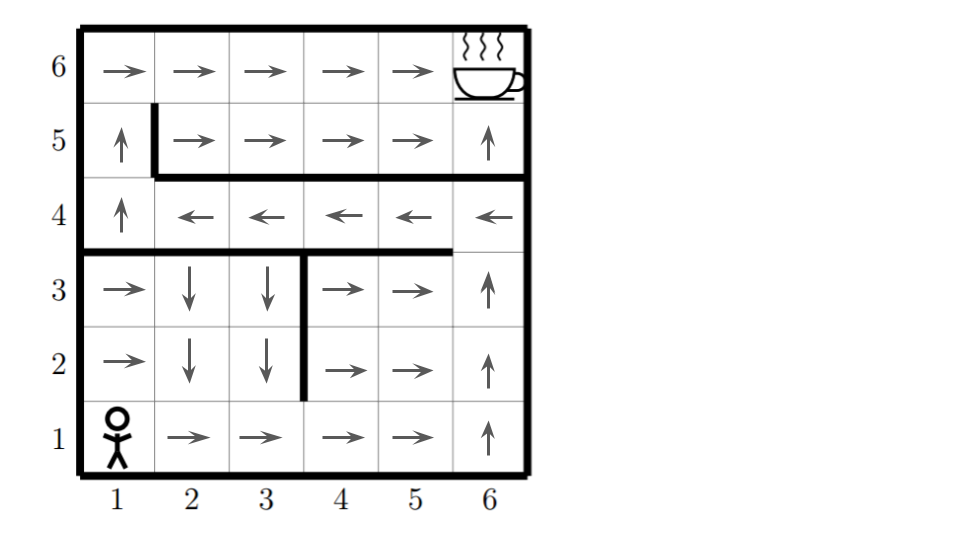
\includegraphics[width=90mm]{policy_ann.png}
\caption{Policy \label{overflow}}
\end{figure}
\item Deterministic
\item In this case, there is no advantage of a stochastic policy. In general, stochastic policies help in exploration in initial stages of learning. 
 
\end{enumerate}

\subsection{Part B}

\begin{enumerate}[label=(\alph*)]
\item Fill in the values for the transition function $P$.\\
    \begin{center}
    \begin{tabular}{|l|l|c|c|c|}\hline
      \multicolumn{2}{|c|}{} &
                               \multicolumn{3}{|c|}{\textbf{s'}}\\\hline
      \textbf{s} & \textbf{a} & (1,3) & (3,2) & (1,4)\\\hline
      (2,2) & up & 0 & 0.1 & 0 \\ \hline
    \end{tabular}
  \end{center}

\item It depends on the optimal policy. Consider the state (5,2). In the previous question, the optimal policy in this state could either be "go right" or "go up". However in the second case, where if we move right, we might end up being in state (5,1) 10\% of the time, the optimal thing to do in state (5,2) is to go up.  
  
\item Yes, it will change. This time, our policy is stochastic so we might end up in low V values in some of the states due to situations described in the previous part.
\end{enumerate}

\subsection{Part C}

\begin{enumerate}[label=(\alph*)]
\item The same reward function as in Part A would work

\item No the agent's policy in the green region will be same as the one in the previous part. This happens as in the green regions, the goal state's reward affects the value of the green states as they are within the horizon. 
  
\item $V_{\pi_a}$ < $V_{\pi_b}$ as in policy b, the expected reward is equal to the reward of the terminal state, which is +10. In policy a, the agent ends up stuck in the state (1,5) as there's a wall beneath it, so it's expected reward is just -1.

\item $V_{\pi_a}$ is same as $V_{\pi_b}$ will be same in the green region, as here the states are affected by the terminal positive reward received by reaching the coffee state. In the blue region, the policies won't converge to anything of interest as there is no reward signal propagating through them. So, the value functions are both equal to -5 (-1 for each step) in the blue region in both cases.  

\end{enumerate}

\section{Problem 2}
\begin{enumerate}[label=(\alph*)]
\item 
For 4*4 env:\\
policy improvement steps : 7 \\
policy evaluation steps : 28 \\ 
time : 0.00603699684143 seconds\\

For 8*8:\\
policy improvement steps : 15\\
policy evaluation steps : 120 \\
time : 0.0430150032043 seconds
\item
4*4
DRDL\\
DLDL\\
RDDL\\
LRRL

8*8
DDDDDDDD\\
DDDRDDDD\\
DDDLDRDD\\
RRRRDLDD\\
RRULDDRD\\
DLLRRDLD\\
DLRULDLD\\
RRULRRRL

\item
Value function plots \\
\begin{figure}[H]
\centering
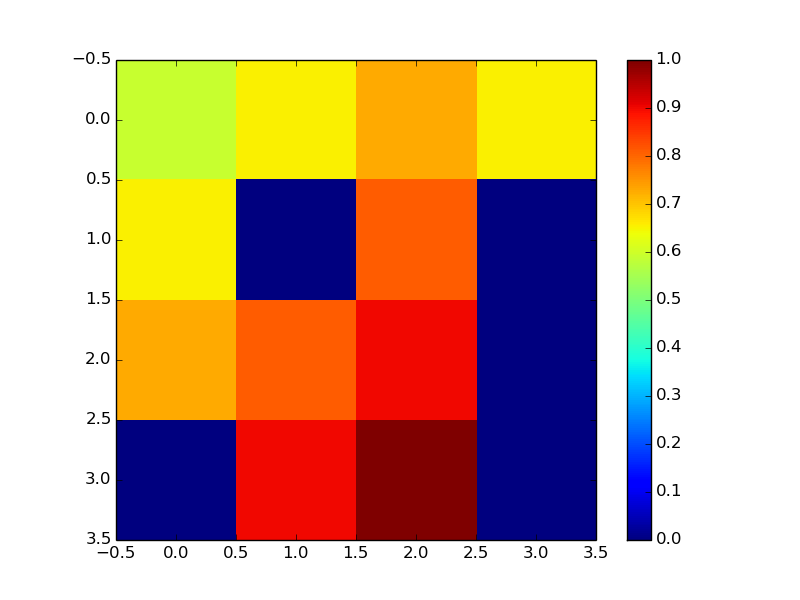
\includegraphics[width=90mm]{4_4.png}
\caption{Value function for 4*4 \label{overflow}}
\end{figure}

\begin{figure}[H]
\centering
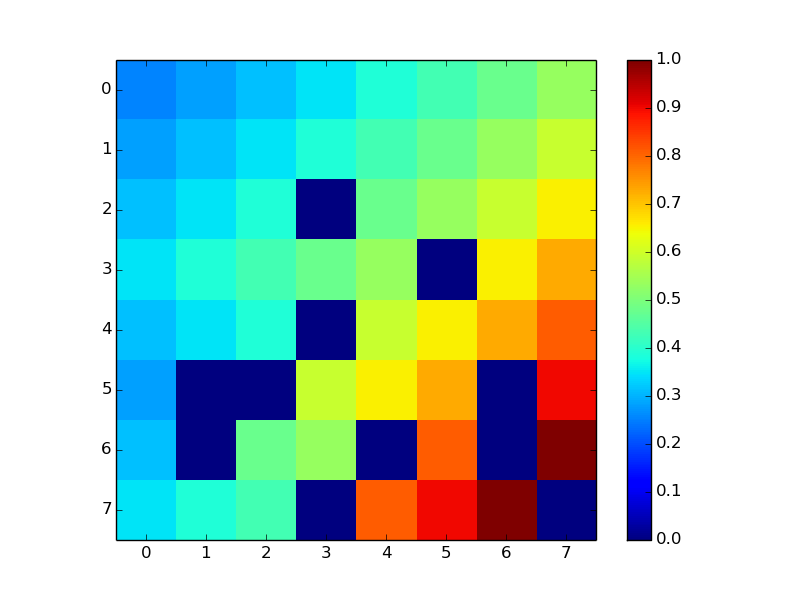
\includegraphics[width=90mm]{8_8.png}
\caption{Value function for 8*8 \label{overflow}}
\end{figure}


\item 
4*4 \\
time : 0.00160002708435s \\
no of iterations : 7

\begin{tabular}{|c|c|c|c|}\hline
0.59033 & 0.65625 & 0.729 & 0.65625 \\\hline
0.65625 & 0.0 & 0.81006 & 0.0 \\\hline
0.729 & 0.81006 & 0.8999 & 0.0 \\\hline
0.0 & 0.8999 & 1.0 & 0.0\\\hline
\end{tabular}

8*8 \\
time : 0.0102798938751s\\
no of iterations : 15

\begin{tabular}{|c|c|c|c|c|c|c|c|}\hline
0.25415 & 0.28247 & 0.31372 & 0.34863 & 0.38745 & 0.43042 & 0.47827 & 0.53125 \\ \hline
0.28247 & 0.31372 & 0.34863 & 0.38745 & 0.43042 & 0.47827 & 0.53125 & 0.59033 \\\hline
0.31372 & 0.34863 & 0.38745 & 0.0 & 0.47827 & 0.53125 & 0.59033 & 0.65625 \\\hline
0.34863 & 0.38745 & 0.43042 & 0.47827 & 0.53125 & 0.0 & 0.65625 & 0.729 \\\hline
0.31372 & 0.34863 & 0.38745 & 0.0 & 0.59033 & 0.65625 & 0.729 & 0.81006 \\\hline
0.28247 & 0.0 & 0.0 & 0.59033 & 0.65625 & 0.729 & 0.0 & 0.8999 \\\hline
0.31372 & 0.0 & 0.47827 & 0.53125 & 0.0 & 0.81006 & 0.0 & 1.0 \\\hline
0.34863 & 0.38745 & 0.43042 & 0.0 & 0.81006 & 0.8999 & 1.0 & 0.0\\\hline
\end{tabular}

\item 

Value function plots \\
\begin{figure}[H]
\centering
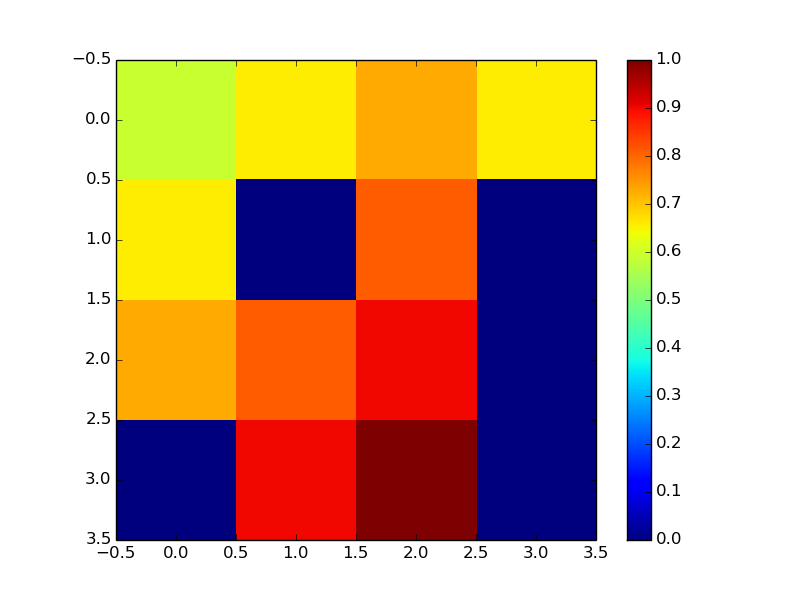
\includegraphics[width=90mm]{4_4_val_iter.png}
\caption{Value function for 4*4 \label{overflow}}
\end{figure}

\begin{figure}[H]
\centering
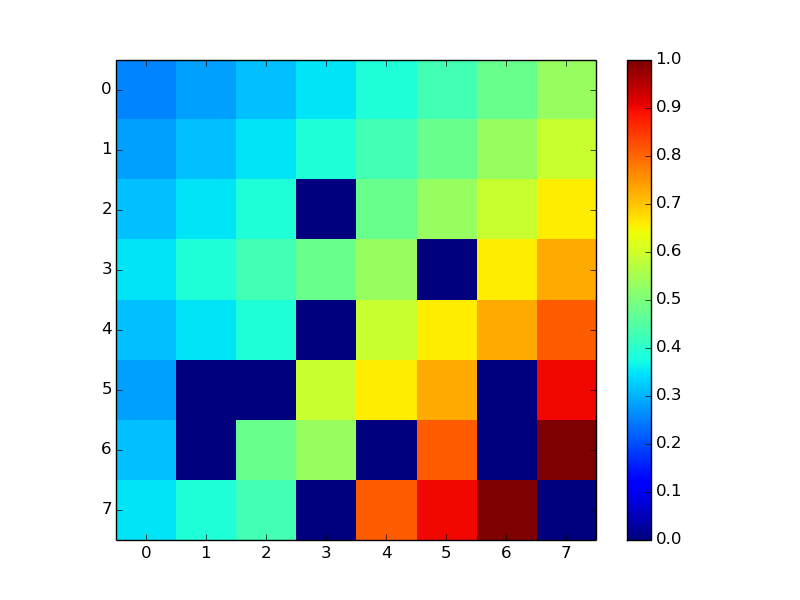
\includegraphics[width=90mm]{8_8_val_iter.png}
\caption{Value function for 8*8 \label{overflow}}
\end{figure}

\item 
Value iteration is faster for both 4*4 and 8*8 cases.
Both take same number of iterations (7 in 4*4 and 15 in 8*8) on the face of it. However, policy iteration runs through the state space twice (once for evaluation - and here it has hidden 28, and 120 iterations respectively - and once for improvement) and thus is slower.

\item
No, there aren't as evident from the plots. Both methods are converging to the same optimal policy. 
\item 
4*4\\
DRDL\\
DLDL\\
RDDL\\
LRRL\\

8*8\\
DDDDDDDD\\
DDDRDDDD\\
DDDLDRDD\\
RRRRDLDD\\
RRULDDRD\\
DLLRRDLD\\
DLRULDLD\\
RRULRRRL\\

\item 

4*4 \\
Discounted reward : 0.59049
Value function : 0.59033

8*8 \\
Discounted reward : 0.25415
Value function : 0.25415

Yes, they both match in both cases
\end{enumerate}


\subsection{Part b}


\begin{enumerate}[label=(\alph*)]
\item

Stochastic 4*4:


time : 0.00626802444458 seconds\\
no of iterations : 23 

\begin{tabular}{|c|c|c|c|}\hline

0.06427 & 0.058075 & 0.072327 & 0.053558 \\\hline
0.088318 & 0.0 & 0.11127 & 0.0 \\\hline
0.14294 & 0.24609 & 0.29883 & 0.0 \\\hline
0.0 & 0.37915 & 0.63867 & 0.0\\\hline
\end{tabular}

Stochastic 8*8

time : 0.0266909599304s 
no of iterations : 24 

\begin{tabular}{|c|c|c|c|c|c|c|c|}\hline
0.0023136 & 0.0043221 & 0.0077286 & 0.013092 & 0.020477 & 0.028015 & 0.03537 & 0.039001 \\\hline
0.0023823 & 0.0040703 & 0.0070953 & 0.01255 & 0.0224 & 0.032623 & 0.046082 & 0.054413 \\\hline
0.0020695 & 0.0030708 & 0.0041771 & 0.0 & 0.022888 & 0.036011 & 0.065063 & 0.082092 \\\hline
0.0017881 & 0.0025864 & 0.0040016 & 0.0067596 & 0.018829 & 0.0 & 0.089783 & 0.12744 \\\hline
0.0013294 & 0.001647 & 0.0016947 & 0.0 & 0.033356 & 0.060883 & 0.10754 & 0.20825 \\\hline
0.00068188 & 0.0 & 0.0 & 0.01059 & 0.031891 & 0.062469 & 0.0 & 0.35913 \\\hline
0.00040483 & 0.0 & 0.001277 & 0.0035591 & 0.0 & 0.11554 & 0.0 & 0.62988 \\\hline
0.0003438 & 0.00044703 & 0.0007329 & 0.0 & 0.13818 & 0.32251 & 0.61426 & 0.0\\\hline
\end{tabular}


\item
Value function plots \\
\begin{figure}[H]
\centering
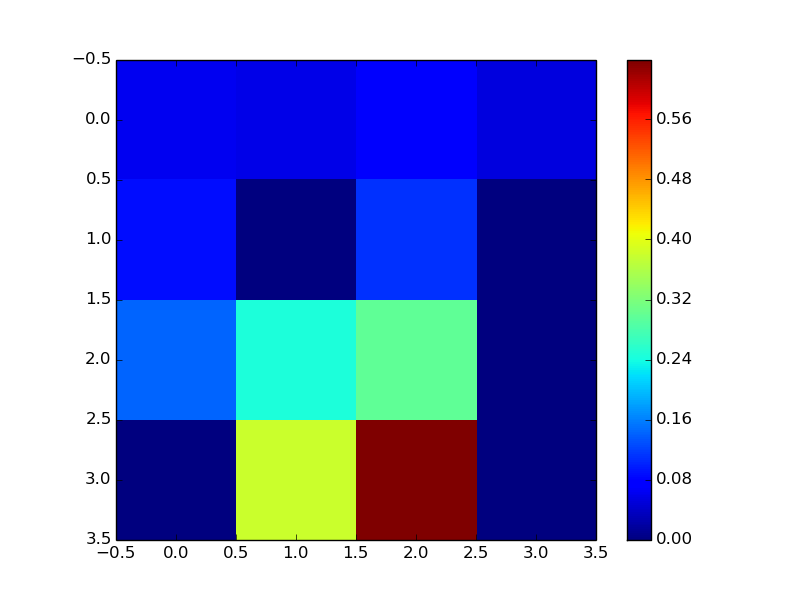
\includegraphics[width=90mm]{4_4_stochastic_val_iter.png}
\caption{Value function for 4*4 \label{overflow}}
\end{figure}

\begin{figure}[H]
\centering
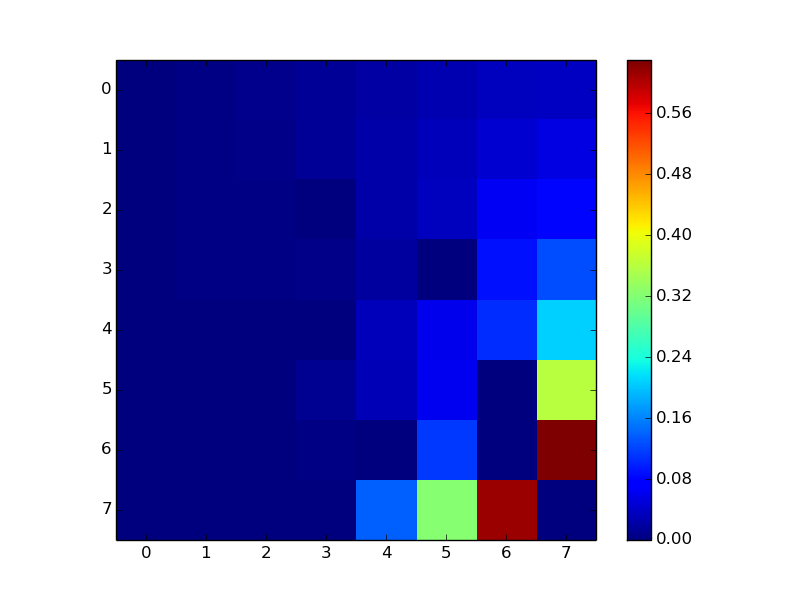
\includegraphics[width=90mm]{8_8_stochastic_val_iter.png}
\caption{Value function for 8*8 \label{overflow}}
\end{figure}


\item
LULU\\
LLLL\\
UDLL\\
LRDL\\

DRRRRRRR\\
URRURRRD\\
URLLRURD\\
UUUDLLRD\\
UULLRDUR\\
LLLDULLR\\
LLDLLLLR\\
RDLLDDDL\\

\item

Yes, the optimal policy differs as compared to the deterministic case. 
\\
Deterministic :\\
DRDL\\
DLDL\\
RDDL\\
LRRL\\

Stochastic:\\
LULU\\
LLLL\\
UDLL\\
LRDL\\

Environment:\\
SFFF\\
FHFH\\
FFFH\\
HFFG\\

Consider the tile to the left of the goal state. In the deterministic cases, the policy is go Right at this state as the agent will always end up in the goal state. 

However, in the stochastic case, the policy is to go Down. This is because, if it goes down, it has a 33\% chance of going to the goal state. If it goes left by chance, the policy on that tile is to go Right, so it will end up in the tile next to the goal state again. 

\item 

4*4 \\
mean cumulative discount reward over 100 steps : 0.00738
value function : 0.06427

8*8\\
mean cumulative discount reward over 100 steps :0.00437
value function : 0.00231

Over infinite data, we can expect the mean cumulative discounted reward to match the value function, but right now it doesn't completely as we're just doing 100 episodes. 

\end{enumerate}



\subsection{Part C}
\begin{enumerate}[label=(\alph*)]

\item Value function plot:
\begin{figure}[H]
\centering
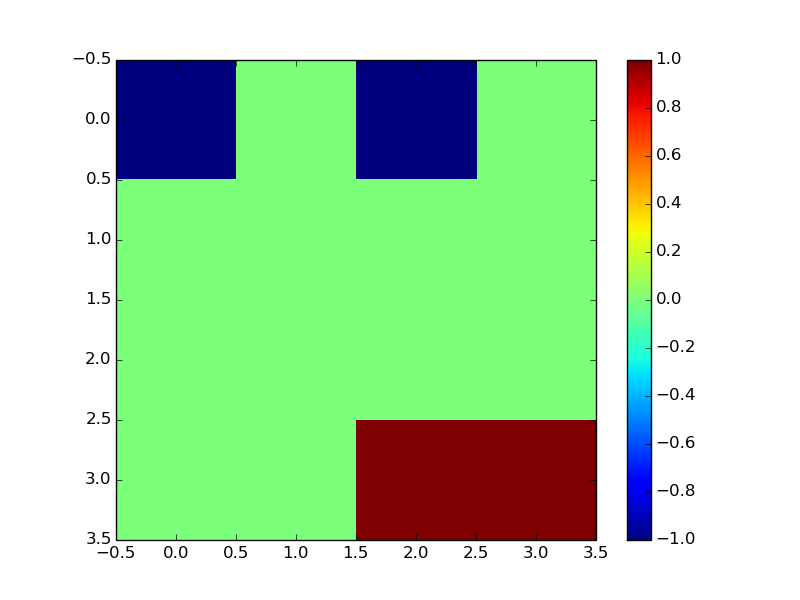
\includegraphics[width=90mm]{4_4_neg_val_iter.png}
\caption{Value function for 4*4 \label{overflow}}
\end{figure}


\item
Yes, it is different, as is evident from the above plot

\item
DDLD\\
RLLL\\
DURL\\
LLRL

Environment:\\
SFFF\\
FHFH\\
FFFH\\
HFFG

We can see that the agent is driving into the holes. 

\item
Positive reward policy:\\
DRDL\\
DLDL\\
RDDL\\
LRRL

Hence, the optimal policy is indeed different as this time the agent is choosing to move towards the hole tiles as they have zero reward whereas the ones which are frozen have -1 reward. 

\end{enumerate}

\section{Problem 3}
Please see the code.

\section{Problem 4}
\begin{enumerate}[label=(\alph*)]
\item From the Contraction Mapping Theorem, we know that for any metric space $V$ that is closed under an operator $T(v)$, T converges to a unique fixed point, if T is a $\gamma$-contraction.
Hence, we need to show that the value iteration operator is indeed a contraction:

We can write the Bellman optimality backup in matrix form as:

\begin{align*}
\lVert F(u)-F(v) \rVert_{\infty} &= \lVert max_{a \in A}(R^a+\gamma P^au) - max_{a \in A}(R^a+\gamma P^av) \rVert_{\infty}\\
&\leq  max_{a \in A}(\lVert R^a+\gamma P^au - R^a-\gamma P^av \rVert_{\infty})\\
&\leq max_{a \in A}(\lVert\gamma P^a (u-v)\rVert_{\infty})\\
&\leq \gamma * max_{a \in A}(P^a \lVert(u-v)\rVert_{\infty})\\
&\leq \gamma * \lVert(u-v)\rVert_{\infty} * max_{a \in A}(P^a)\\
&\leq \gamma \lVert u-v \rVert_{\infty}
\end{align*}
\item
At each iteration, we're doing $V_{k+1}=FV_k$.\\
Let's write the contraction mapping theorem wrt $V^k=(F^*)^kV_0$ and $V^*$ as k approaches infinity:
\begin{align*}
\lVert V^k- V^* \rVert_{\infty} 
= \lVert FV^{k-1}- FV^* \rVert_{\infty} \leq \gamma \lVert V^{k-1}- V^* \rVert_{\infty} \\
= \gamma \lVert FV^{k-2}- FV^* \rVert_{\infty}  \leq \gamma^2 \lVert V^{k-1}- V^* \rVert_{\infty} \\ ... \\
\leq \gamma^k \lVert V^{0}- V^* \rVert_{\infty} \\  \rightarrow 0 
\end{align*}
as $\gamma$<1.

\item \begin{align*}
  \pi ^*(s) = \argmax _{a \in A} 
    \left(
      \sum _{s' \in S} 
        P(s' | s, a) \left(
          R (s, a, s') + \gamma V ^*( s' )
        \right)
    \right) .
\end{align*}
\end{enumerate}


\end{document}
